% =================== PREAMBLE SNIPPET (put in your preamble) ===================
% \usepackage{booktabs}
% \usepackage{siunitx}
% \usepackage{graphicx}
% \usepackage{subcaption}
% \usepackage{caption}
% \usepackage{float}       % for [H] placement if you want
% \sisetup{detect-all,round-mode=places,round-precision=2}

% Handy macros (edit if needed)
\newcommand{\annfac}{365}
\newcommand{\sampleStart}{2021-01-01}
\newcommand{\sampleEnd}{2024-06-30}
\newcommand{\neutralScale}{0.5}

% =================== RESULTS CHAPTER (paste in body) ===================
\chapter{Results and Evaluation}\label{sec:results}

We use \sampleStart{}–\sampleEnd{} as the data-availability window. The \emph{effective} evaluation start date $t_0$ is configuration-dependent due to warm-up requirements in both components. For each configuration we begin evaluation at its first tradable day $t_0$ (signals on $t$, execution on $t^+$). Annualisation uses factor \annfac{}, costs are reported separately, and the risk-free rate is set to zero. %When comparing multiple configurations, we make clear whether results are computed on each strategy’s own window (per-strategy $t_0$) or on the intersection-aligned window (common $t_0=\max$ of all configurations).


%We evaluate daily close-to-close strategies on \sampleStart{}–\sampleEnd{}.
%Unless otherwise noted, annualization uses factor \annfac{}, costs are reported separately, and portfolios are executed on $t^+$ (first trading day after signal time).










\section{Headline Performance}\label{sec:results:headline}

\begin{table}[t]
\centering
\caption{Headline performance.}
\label{tab:main}
\small
\begin{tabular}{lcc}
\toprule
Metric & Baseline & Overlay (preserves hedge) \\
\midrule
Cumulative Return (\%)     & 59.53 & 132.78 \\
CAGR (\%)                  & 16.28 & 31.38  \\
Volatility (ann., \%)      & 38.09 & 20.06  \\
Sharpe                     & 0.58  & 1.46   \\
Sortino                    & 0.90  & 2.46   \\
Max Drawdown (\%)          & -35.32 & -14.15 \\
Time in Market (\%)        & 43.0  & 43.0   \\
%Risk-free rate (\%)        & 0.0   & 0.0    \\
Final NAV                  & 1.5953 & 2.3278 \\
Active Days (approx.)      & 549   & 549    \\
\bottomrule
\end{tabular}
\end{table}

Table~\ref{tab:main} reports headline performance of the lead--lag hedge. The overlay keeps that hedge and adds regime awareness. The risk--free rate is zero. The overlay delivers a stronger risk--return trade--off. Cumulative return rises from \textbf{59.53\%} to \textbf{132.78\%}. CAGR increases from \textbf{16.28\%} to \textbf{31.38\%} (see Figure~\ref{fig:nav}). Meanwhile, annualised volatility falls from \textbf{38.09\%} to \textbf{20.06\%}. As a result, Sharpe improves from \textbf{0.58} to \textbf{1.46}, and Sortino from \textbf{0.90} to \textbf{2.46}. Drawdowns also ease: the maximum drawdown tightens from \textbf{--35.32\%} to \textbf{--14.15\%}. Importantly, time in market is identical at \textbf{43\%}. So the gains come from better selection and positioning, not from higher exposure. Final NAV rises from \textbf{1.5953} to \textbf{2.3278}. In short, the overlay earns more with materially less risk at the same participation rate.

Figure~\ref{fig:roll_sharpe_6m} plots the rolling 6-month Sharpe. 
The overlay spends more time above 1 and shortens negative spells around 2022, consistent with its faster exit and recovery.


\begin{figure}[t]
\centering
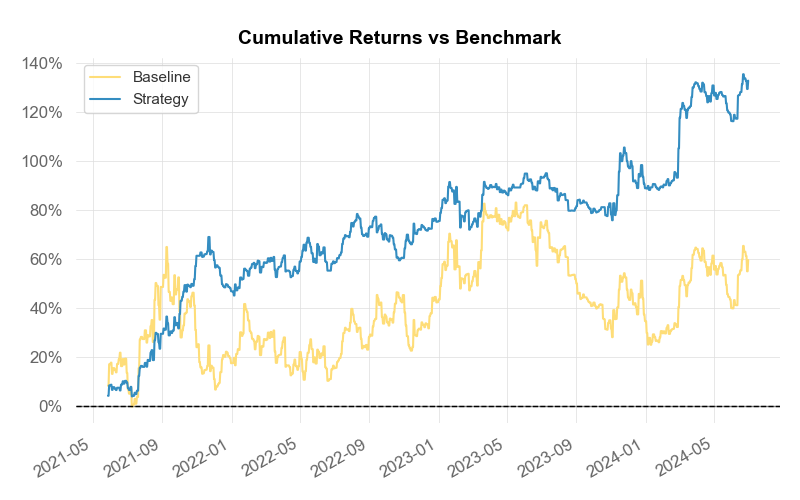
\includegraphics[width=0.9\linewidth]{headline_plots/NAV.png}% <-- put your path
\caption{Cumulative NAV: baseline vs.\ regime overlay.}
\label{fig:nav}
\end{figure}

\begin{figure}[t]
\centering
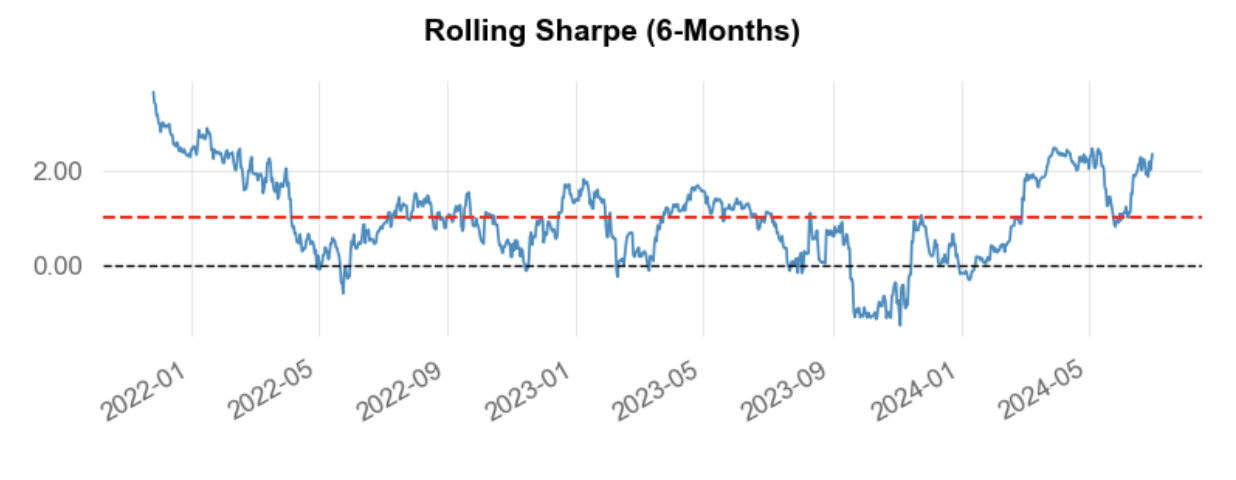
\includegraphics[width=0.9\linewidth]{headline_plots/Rolling_Sharp.png}
\caption{Rolling 6-month Sharpe for the baseline and the Overlay.}
\label{fig:roll_sharpe_6m}
\end{figure}


\begin{table}[t]
\centering
\caption{Drawdown details.}
\label{tab:diag_dd}
\small
\begin{tabular}{lcc}
\toprule
Metric & Baseline & Overlay \\
\midrule
Max DD (\%)          & -35.32 & -14.15 \\
Max DD Date          & 2021-12-03 & 2022-01-05 \\
Max DD Period Start  & 2021-09-10 & 2021-11-24 \\
Max DD Period End    & 2023-01-17 & 2022-07-19 \\
Longest DD Days      & 495 & 238 \\
\bottomrule
\end{tabular}
\end{table}

Table~\ref{tab:diag_dd} details the drawdown. The overlay cuts the peak--to--trough loss from \textbf{--35.32\%} to \textbf{--14.15\%}. It also halves time under water from \textbf{495} to \textbf{238} days. The baseline’s worst episode is long and persistent (\textbf{2021-09-10} to \textbf{2023-01-17}; trough on \textbf{2021-12-03}) and spans the 2022 downturn. The overlay’s worst spell starts later (\textbf{2021-11-24}), bottoms quickly (\textbf{2022-01-05}), and ends by mid-\textbf{2022} (\textbf{2022-07-19}). In other words, it absorbs the early-2022 selloff but exits and recovers faster. Net effect: a softer left tail and a shorter recovery horizon, consistent with the higher risk-adjusted performance.

\begin{table}[t]
\centering
\caption{EOY returns vs.\ baseline. Multiplier $=$ Strategy / Baseline; negative means opposite signs.}
\label{tab:eoy}
\small
\begin{tabular}{lrrrr}
\toprule
Year & Baseline & Strategy & Multiplier & Won \\
\midrule
2021 & 16.28\% & 46.77\% & 2.87  & $+$ \\
2022 & 21.22\% & 19.36\% & 0.91  & $-$ \\
2023 & $-5.42$\% & 7.79\% & $-1.44$ & $+$ \\
2024 & 18.54\% & 23.27\% & 1.26  & $+$ \\
\bottomrule
\end{tabular}
\end{table}

Table~\ref{tab:eoy} compares year-end returns and the multiplier (Strategy/Baseline). The overlay wins in \textbf{three of four} years---\textbf{2021}, \textbf{2023}, and \textbf{2024 (YTD)}---with multipliers of \textbf{2.87}, \textbf{-1.44}, and \textbf{1.26}. The negative multiplier in 2023 signals a sign flip (baseline \(-5.42\%\) vs.\ strategy \(+7.79\%\)). In \textbf{2022}, the multiplier is \textbf{0.91}, a mild shortfall. Overall, the overlay adds value when the baseline struggles and still provides an edge in rising markets.

\begin{table}[t]
\centering
\caption{Top-5 by Sharpe compared with baseline strategy.}
\label{tab:top5_sharpe_params}
\small
\begin{tabular}{lccccccc}
\toprule
Strategy (params) & Sharpe & CAGR & Vol (ann) & MaxDD & Calmar & Alpha (ann) & WinRate \\
\midrule
$n\_steps, n\_paths=5, 20$ & 1.460 & 0.314 & 0.201 & -0.141 & 2.161 & 0.212 & 0.215 \\
$n\_steps, n\_paths=5, 16$ & 1.006 & 0.217 & 0.218 & -0.207 & 1.046 & 0.126 & 0.216 \\
$n\_steps, n\_paths=15, 12$ & 0.892 & 0.150 & 0.173 & -0.173 & 0.863 & 0.112 & 0.155 \\
$n\_steps, n\_paths=15, 16$ & 0.853 & 0.154 & 0.188 & -0.155 & 0.994 & 0.100 & 0.157 \\
$n\_steps, n\_paths=5, 8$  & 0.816 & 0.161 & 0.210 & -0.192 & 0.841 & 0.095 & 0.214 \\
\hline
Baseline & 0.580 & 0.163 & 0.380 & -0.353 & 0.440 & 0.000 & 0.219 \\
\bottomrule
\end{tabular}
\end{table}


\section{Strategy selection and performance}\label{sec:results:top5}


% In your preamble:
% \usepackage{graphicx}

\begin{figure}[t]
  \centering
  % If you saved to images/top5_nav_union.png:
  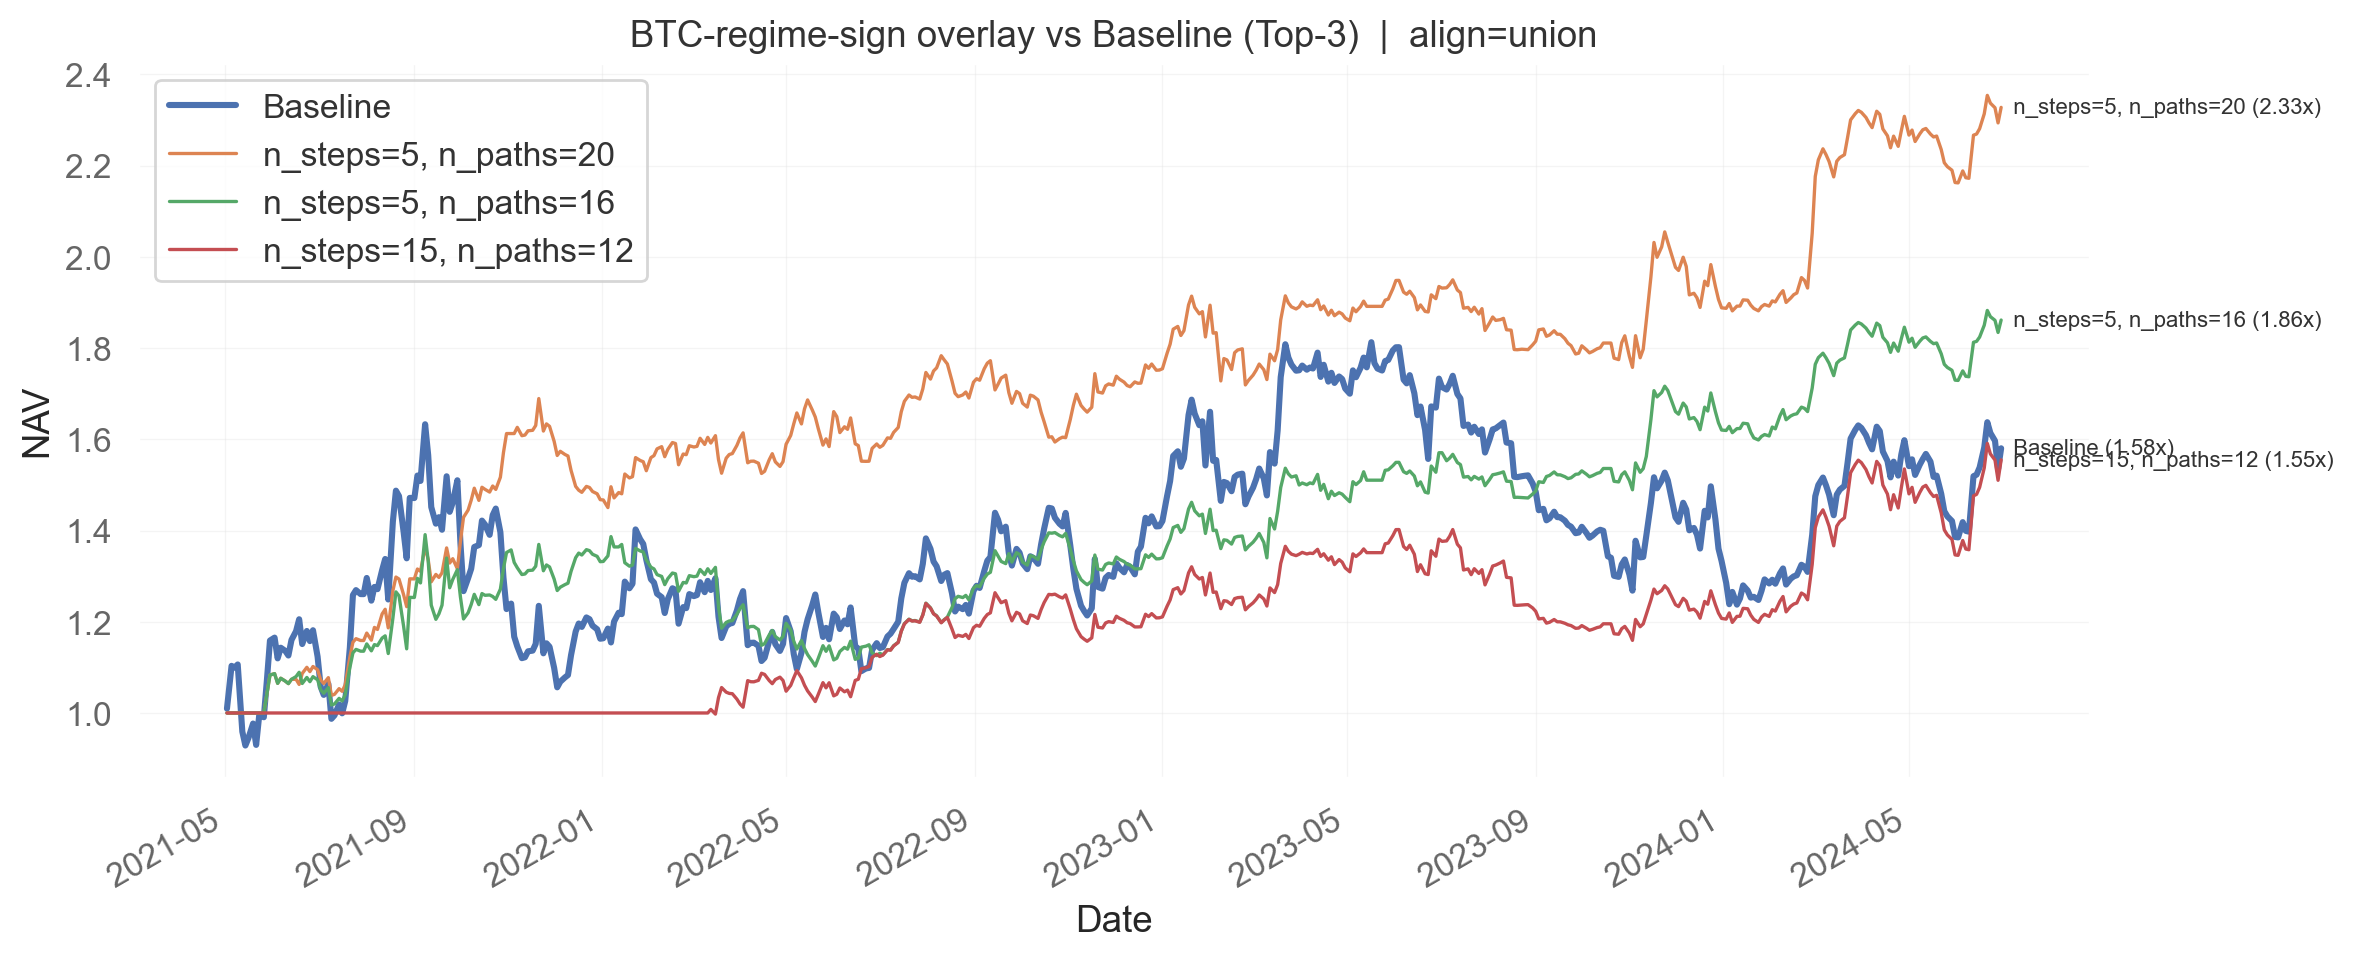
\includegraphics[width=\linewidth]{headline_plots/top3_nav_union.png}
  \caption{Top-3 NAV vs. Baseline (union-aligned). Values annotated at the last date indicate final NAV multiples.}
  \label{fig:top5_nav_union}
\end{figure}

First, we evaluate candidate parameterisations in a \emph{strict walk-forward} setup, train only on past windows and label only the current group. Then we rank each configuration by Sharpe. For context, we also report the Baseline. Throughout, we use a unified daily calendar with a crypto annualisation factor of 365. We align returns from the \emph{signal day} to the \emph{next trading day}. Rates are in decimals (e.g., 0.20 = 20\%). See Table~\ref{tab:top5_sharpe_params}.

Short windows with more paths perform best. In particular, \(n_{\text{steps}}=5\) with \(n_{\text{paths}}\in\{16,20\}\) leads. The top configuration, \(n_{\text{steps}}=5, n_{\text{paths}}=20\), reaches a Sharpe of 1.44 with annualised volatility of 0.20, maximum drawdown \(-0.14\), and Calmar 2.16. By contrast, the Baseline records a Sharpe of 0.56 and a Calmar of 0.44. Meanwhile, mid-range windows—such as \(n_{\text{steps}}=15\) with \(n_{\text{paths}}\in\{12,16\}\)—also offer a solid return-risk trade-off.

We assess significance against zero using Newey--West (HAC, Bartlett kernel; data-driven lag) t-statistics \cite{NeweyWest1994} on daily excess returns (See Appendix \ref{sec:newey-west}).
We then build 95\% moving-block bootstrap confidence intervals (block = 10 days, $B=2000$) for annualized return and Sharpe on the unified calendar.
Table~\ref{tab:sig_compact} reports the Baseline and the top five overlays by Sharpe.
As shown, \emph{Overlay (5,20)} is significant versus zero; both confidence intervals lie strictly above zero.
\emph{Overlay (5,16)} is marginally significant.
By contrast, the Baseline and the remaining overlays are not significant at the 5\% level, with intervals overlapping zero.

\begin{table}[t]
\centering
\caption{Significance vs.\ zero: NW $t$ on daily mean excess, and 95\% block-bootstrap CIs. Rates in decimals (e.g., 0.20 = 20\%).}
\label{tab:sig_compact}
\small
\begin{tabular}{lccccc}
\toprule
Strategy & NW $t$ (mean) & AnnRet (pt) & AnnRet [2.5\%,97.5\%] & Sharpe (pt) & Sharpe [2.5\%,97.5\%] \\
\midrule
Baseline        & 1.29 & 0.24 & [$-0.18$, $0.90$] & 0.58 & [$-0.35$, $1.80$] \\
Overlay (5,20)  & 2.67 & 0.33 & [$0.08$,  $0.64$] & 1.46 & [$0.48$,  $2.48$] \\
Overlay (5,16)  & 2.01 & 0.24 & [$0.01$,  $0.54$] & 1.00 & [$0.13$,  $2.10$] \\
Overlay (15,12) & 1.58 & 0.15 & [$-0.05$, $0.40$] & 0.89 & [$-0.20$, $1.96$] \\
Overlay (15,16) & 1.54 & 0.16 & [$-0.05$, $0.43$] & 0.85 & [$-0.18$, $1.88$] \\
Overlay (5,8)   & 1.53 & 0.17 & [$-0.07$, $0.47$] & 0.81 & [$-0.25$, $1.90$] \\
\bottomrule
\end{tabular}
\end{table}

Several other settings (e.g., \(n_{\text{steps}}\in\{8,10\}\)) are mediocre or negative in this sample and are omitted. In practice, implementation should also account for switching frequency and transaction costs (see the switch-rate diagnostics), since these frictions affect net returns and capacity. Overall, the walk-forward state signal, when combined with our overlay, improves risk-adjusted performance, with “shorter steps + more paths” as the most effective pattern in this dataset.


\section{Transaction-cost modeling and impact}\label{sec:tc}

We model transaction costs in a simple, transparent way that matches our portfolio construction and evaluation. First, on each trading day \(t\) we form target portfolio weights \(w_t\) (long equal-weight followers; short equal-weight leaders). Next, we proxy trading volume with the absolute change in target weights.
\[
\text{turnover}_t = \sum_i \lvert w_{t,i} - w_{t-1,i}\rvert.
\]
We then apply a per-side fee of \(c\) basis points to this turnover, which yields the daily cost
\[
\text{cost}_t = (c\times 10^{-4})\;\text{turnover}_t.
\]
Consequently, we compute net returns in \emph{simple-return} space as
\(r^{\text{net}}_t = r^{\text{gross}}_t - \text{cost}_t\).
We charge for the first trade (initial portfolio formation) and use the \emph{target-diff} mechanic. %For completeness, a \emph{full-rebalance} variant that also offsets drift back to equal weights produces higher costs and is reported when noted.

\begin{table}
\caption{Baseline transaction-cost sensitivity (per side, applied to target-weight changes).}
\label{tab:baseline_tc}
\small
\centering
\begin{tabular}{rrrrr}
\toprule
Cost (bps/side) & Sharpe & AnnRet (\%) & Vol (\%) & MaxDD (\%) \\
\midrule
5   & 0.323  & 5.07   & 40.98 & -42.36 \\
10  & -0.015 & -8.56  & 40.99 & -58.57 \\
25  & -1.026 & -39.77 & 41.15 & -86.30 \\
\bottomrule
\end{tabular}
\end{table}

\begin{table}
\caption{Transaction-cost sensitivity. Costs are per side, applied to target-weight changes.}
\label{tab:tc_sensitivity_reduced}
\small
\centering
\begin{tabular}{lrrrr}
\toprule
Strategy (params) & Sharpe & AnnRet (\%) & Vol (\%) & MaxDD (\%) \\
\midrule
\multicolumn{5}{l}{\emph{Cost = 5 bps/side}}\\
\params{5}{20} & 1.052 & 26.82 & 25.70 & -22.98 \\
\params{5}{16} & 0.628 & 14.24 & 26.86 & -34.98 \\
\params{15}{12} & 0.475 & 9.45 & 26.12 & -31.18 \\
\params{15}{16} & 0.561 & 11.88 & 25.96 & -27.17 \\
\params{5}{8} & 0.485 & 9.81 & 26.50 & -26.90 \\
\addlinespace
\multicolumn{5}{l}{\emph{Cost = 10 bps/side}}\\
\params{5}{20} & 0.672 & 15.03 & 25.68 & -32.08 \\
\params{5}{16} & 0.289 & 4.28 & 26.82 & -39.22 \\
\params{15}{12} & 0.122 & -0.19 & 26.13 & -36.51 \\
\params{15}{16} & 0.197 & 1.78 & 25.96 & -33.31 \\
\params{5}{8} & 0.103 & -0.76 & 26.50 & -34.76 \\
\addlinespace
\multicolumn{5}{l}{\emph{Cost = 25 bps/side}}\\
\params{5}{20} & -0.466 & -14.21 & 25.79 & -65.20 \\
\params{5}{16} & -0.732 & -20.73 & 26.84 & -63.57 \\
\params{15}{12} & -0.931 & -24.35 & 26.28 & -68.04 \\
\params{15}{16} & -0.892 & -23.39 & 26.07 & -66.77 \\
\params{5}{8} & -1.038 & -26.80 & 26.62 & -68.02 \\
\bottomrule
\end{tabular}
\end{table}

Costs erode performance roughly in line with annualised turnover. For the Baseline (Table~\ref{tab:baseline_tc}), sharpe drops from \(0.58\) at \(0\) bps to \(0.32\) at \(5\) bps, and turns negative by \(10\) bps. Therefore, the break-even lies between \(5\) and \(10\) bps under the \emph{target-diff} mechanic. By contrast, the best overlay configurations (Table~\ref{tab:tc_sensitivity_reduced}) suffer a milder hit thanks to lower average daily turnover (\(\sim1.16\)–\(1.30\) vs.\ Baseline \(1.77\)). For example, \(n_{\text{steps}}=5, n_{\text{paths}}=20\) remains attractive at \(5\)–\(10\) bps (Sharpe \(1.05 \to 0.67\)), yet performance compresses sharply beyond \(25\) bps. As expected, volatility is largely unchanged across bps grids, while maximum drawdowns deepen as net returns are shaved each day. At high frictions, all configurations become economically unviable, and NAVs converge toward unity.


% --------- OPTIONAL (comment out if not needed now) ----------
% \subsection{Ablations (compact)}
% \begin{table}[t]
% \centering
% \caption{Key ablations. Effect on Sharpe / MDD / turnover.}
% \begin{tabular}{lrrr}
% \toprule
% Variant & $\Delta$Sharpe & $\Delta$Max DD (pp) & $\Delta$Turnover (pp/day) \\
% \midrule
% No preserve-hedge &  &  &  \\
% No apply-to-leaders &  &  &  \\
% abs\_rel\_quantile=0.8 &  &  &  \\
% \bottomrule
% \end{tabular}
% \end{table}
